\chapter{関連技術}
本章では、本研究で使用したデバイスや関連した研究について述べる.
また,振動刺激がユーザーに与える影響についての関連研究を紹介する.
%%%%%%%%%%%%%%%%%%%%%%%%%%%%%%%%%%%%%%%%%%%%%%%%%%%%%%%%%%%%%%%%%%%%%%%
\begin{comment}
\begin{textblock}{6}(14.5, 22)
  ←図のキャプションは図の下
\end{textblock}
\end{comment}
%%%%%%%%%%%%%%%%%%%%%%%%%%%%%%%%%%%%%%%%%%%%%%%%%%%%%%%%%%%%%%%%%%%%%%%

% 




\section{Vive Cosmos Elite}

\begin{figure}[h]
\centering
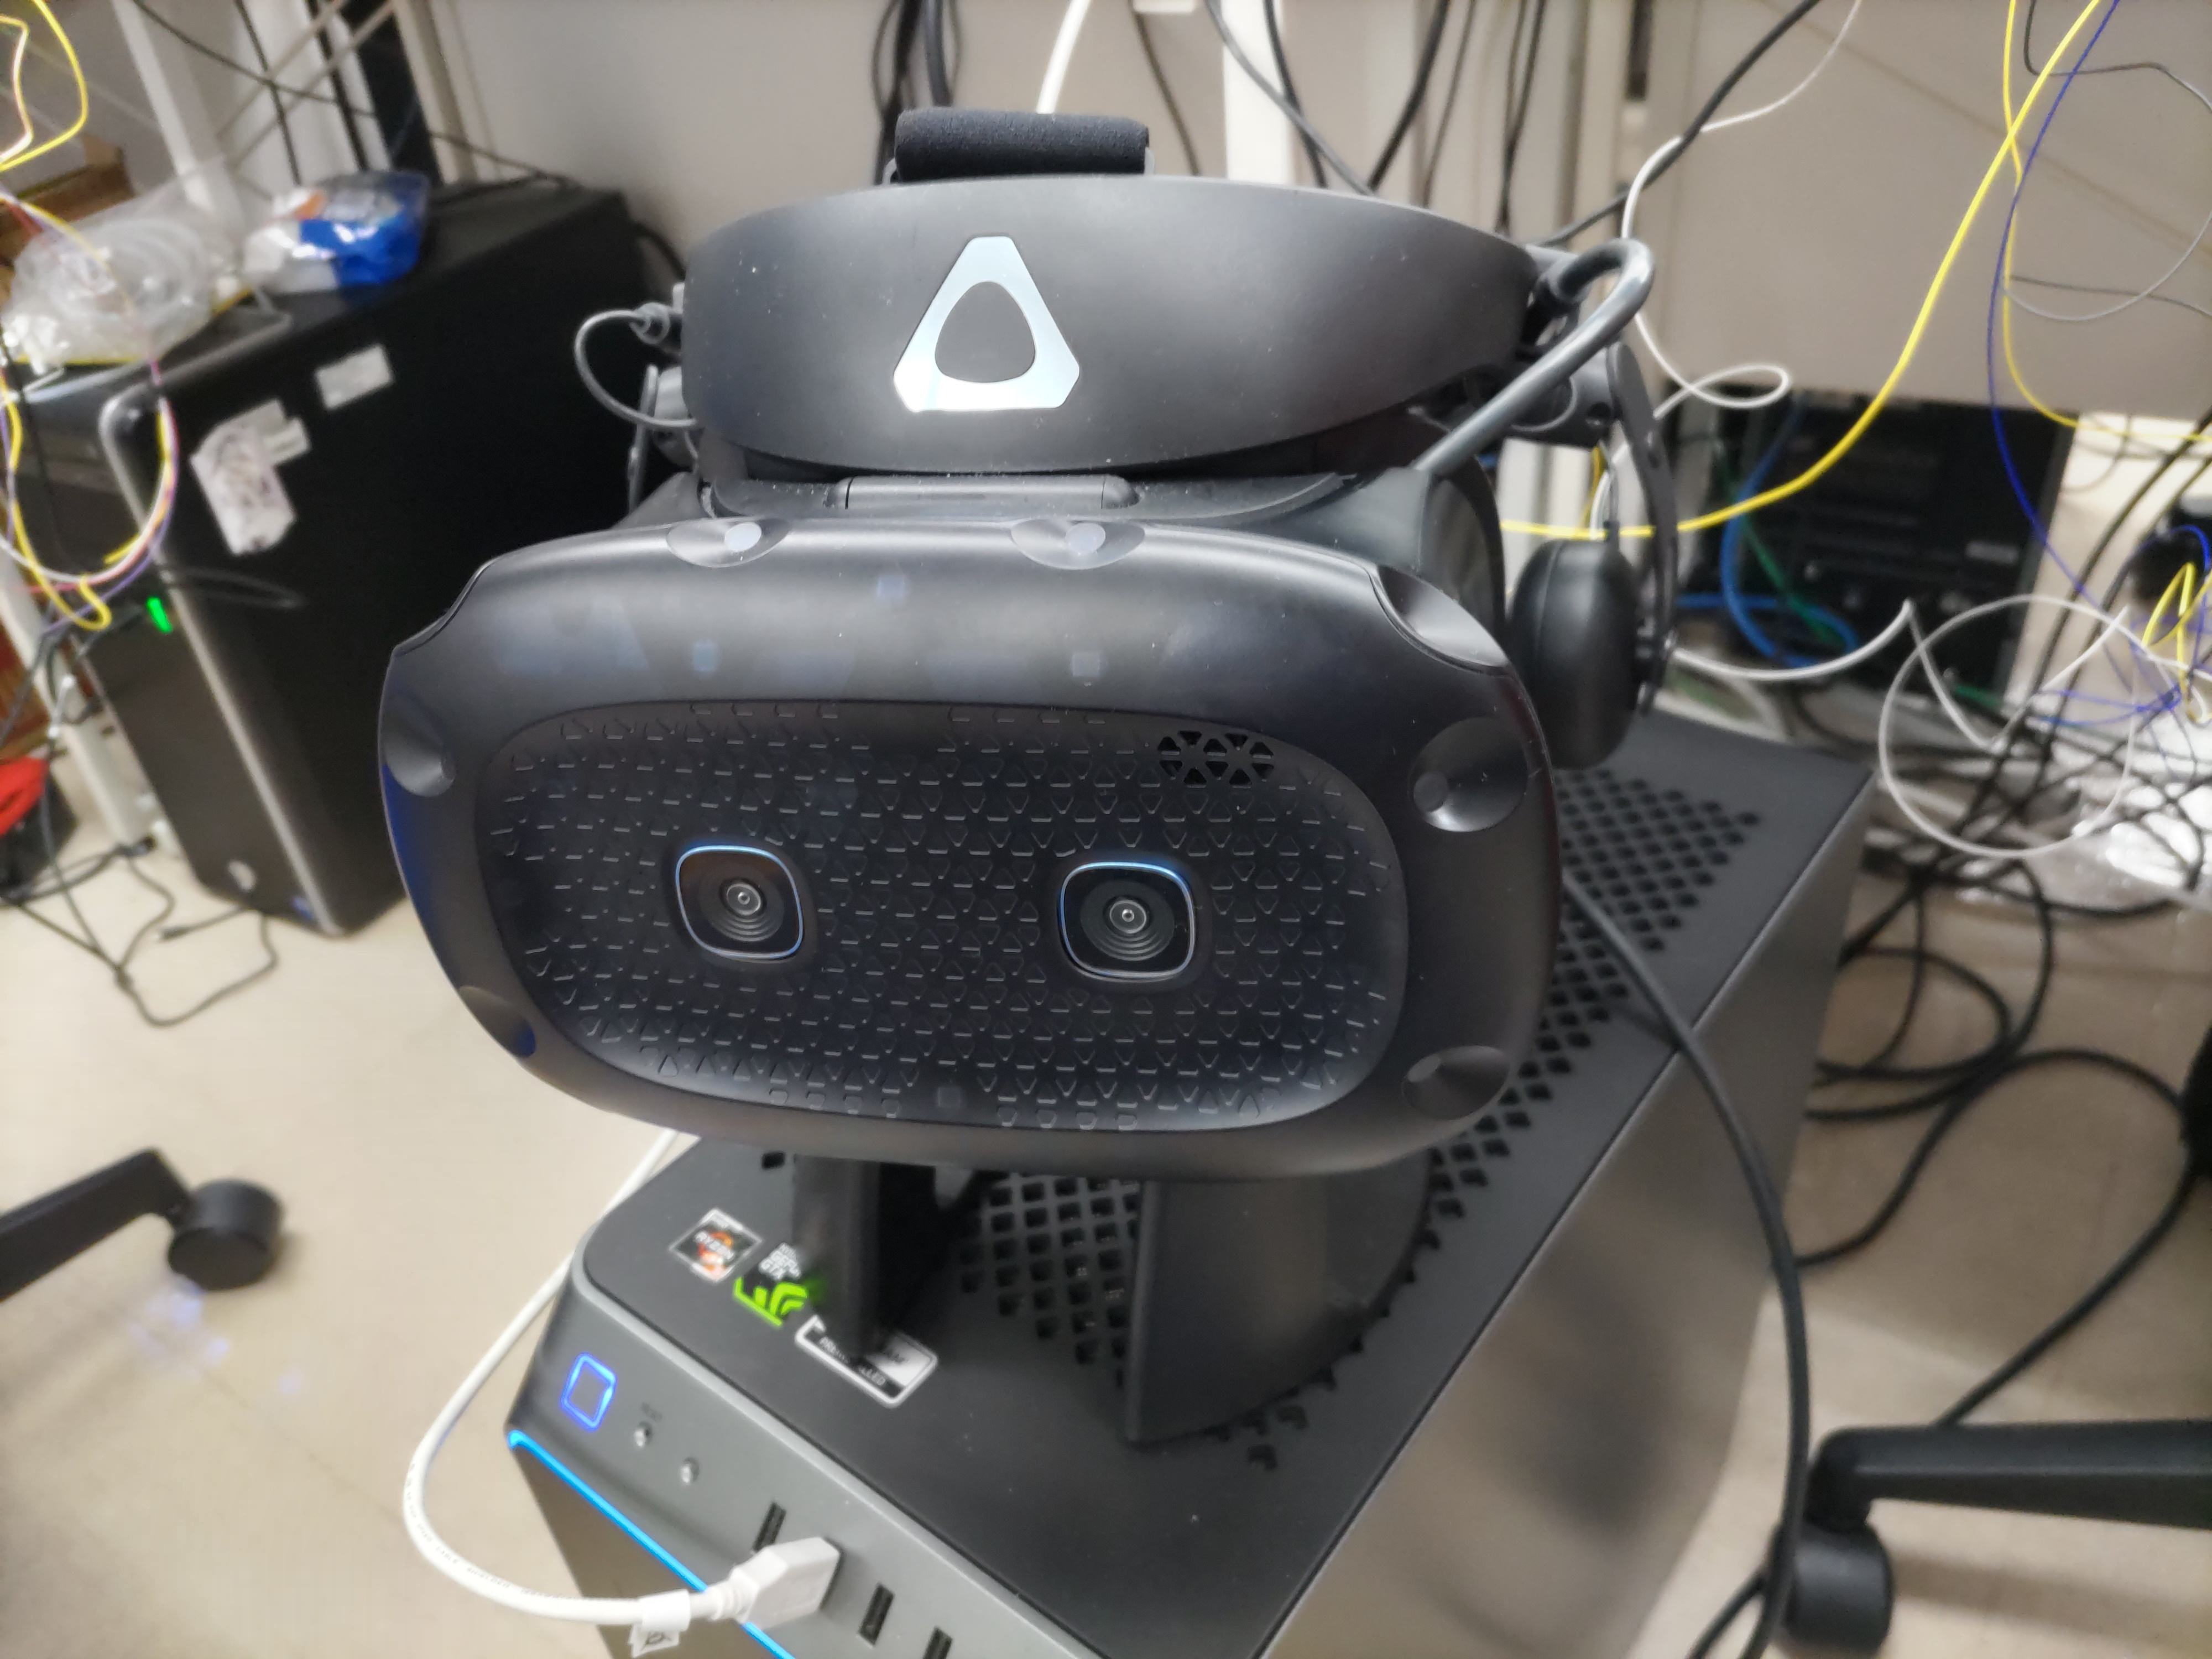
\includegraphics[clip,width=8cm]{./fig/VIVE.JPG}
\caption{VIVE Cosmos Elite}\label{VIVE}
\end{figure}
本研究で使用したVIVEcosmosEliteを\figref{VIVE}に示す.
VIVEcosmosEliteはHTCVIVEが開発したヘッドマウントディスプレイの1つである.
VR空間内での座標と方向を取得を取得し,HMD にVR空間を投影する.

\newpage

\section{振動モーター}

\begin{figure}[h]
\centering
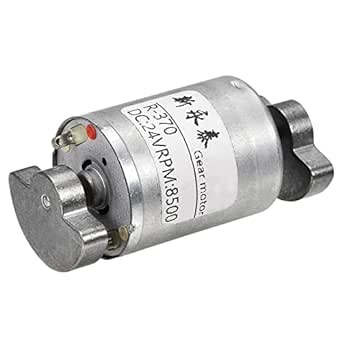
\includegraphics[clip,width=8cm]{./fig/Motor.jpg}
\caption{振動モーター}\label{motor}
\end{figure}

本研究では,ユーザーに振動刺激を与えるために振動モーターを用いる.使用した振動モーターは\figref{motor}に示す.

\section{押しボタン}
\begin{figure}[h]
\centering
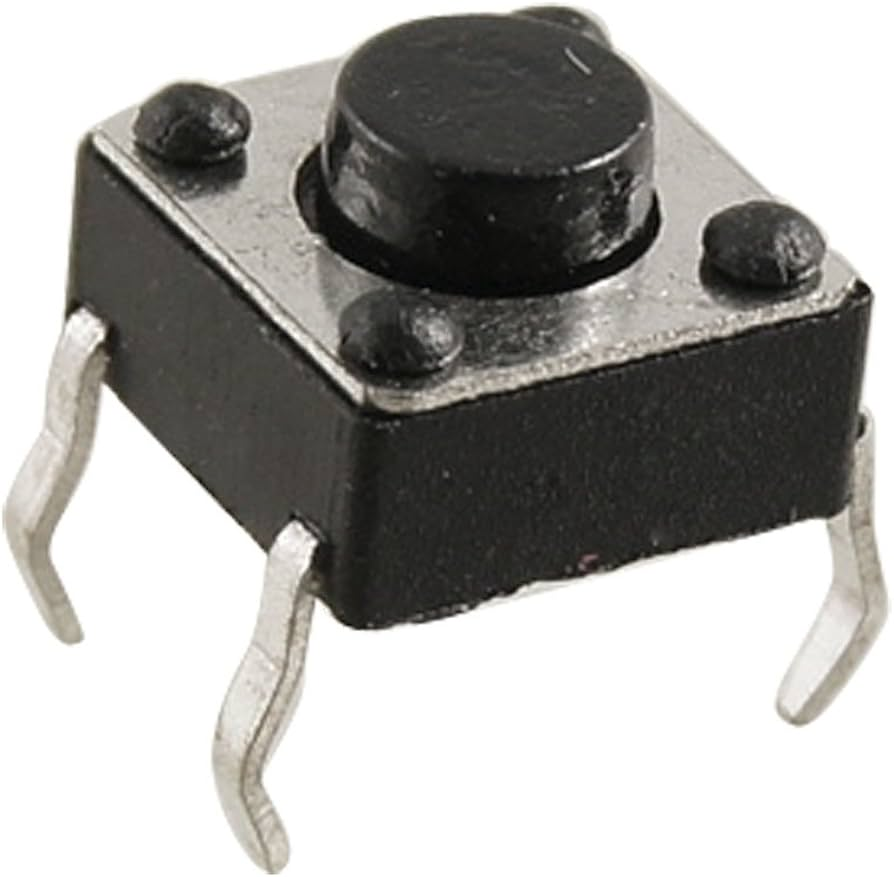
\includegraphics[clip,width=5cm]{./fig/push.jpg}
\caption{押しボタン}\label{push}
\end{figure}

本研究では押しボタンを押すことでarduinoに信号を送り,unity上の視覚エフェクトやモータードライバを作動させる.
任意のタイミングでユーザーにボタンを押させることで没入感の低下を防止している.


\section{Arduino}

\begin{figure}[h]
\centering
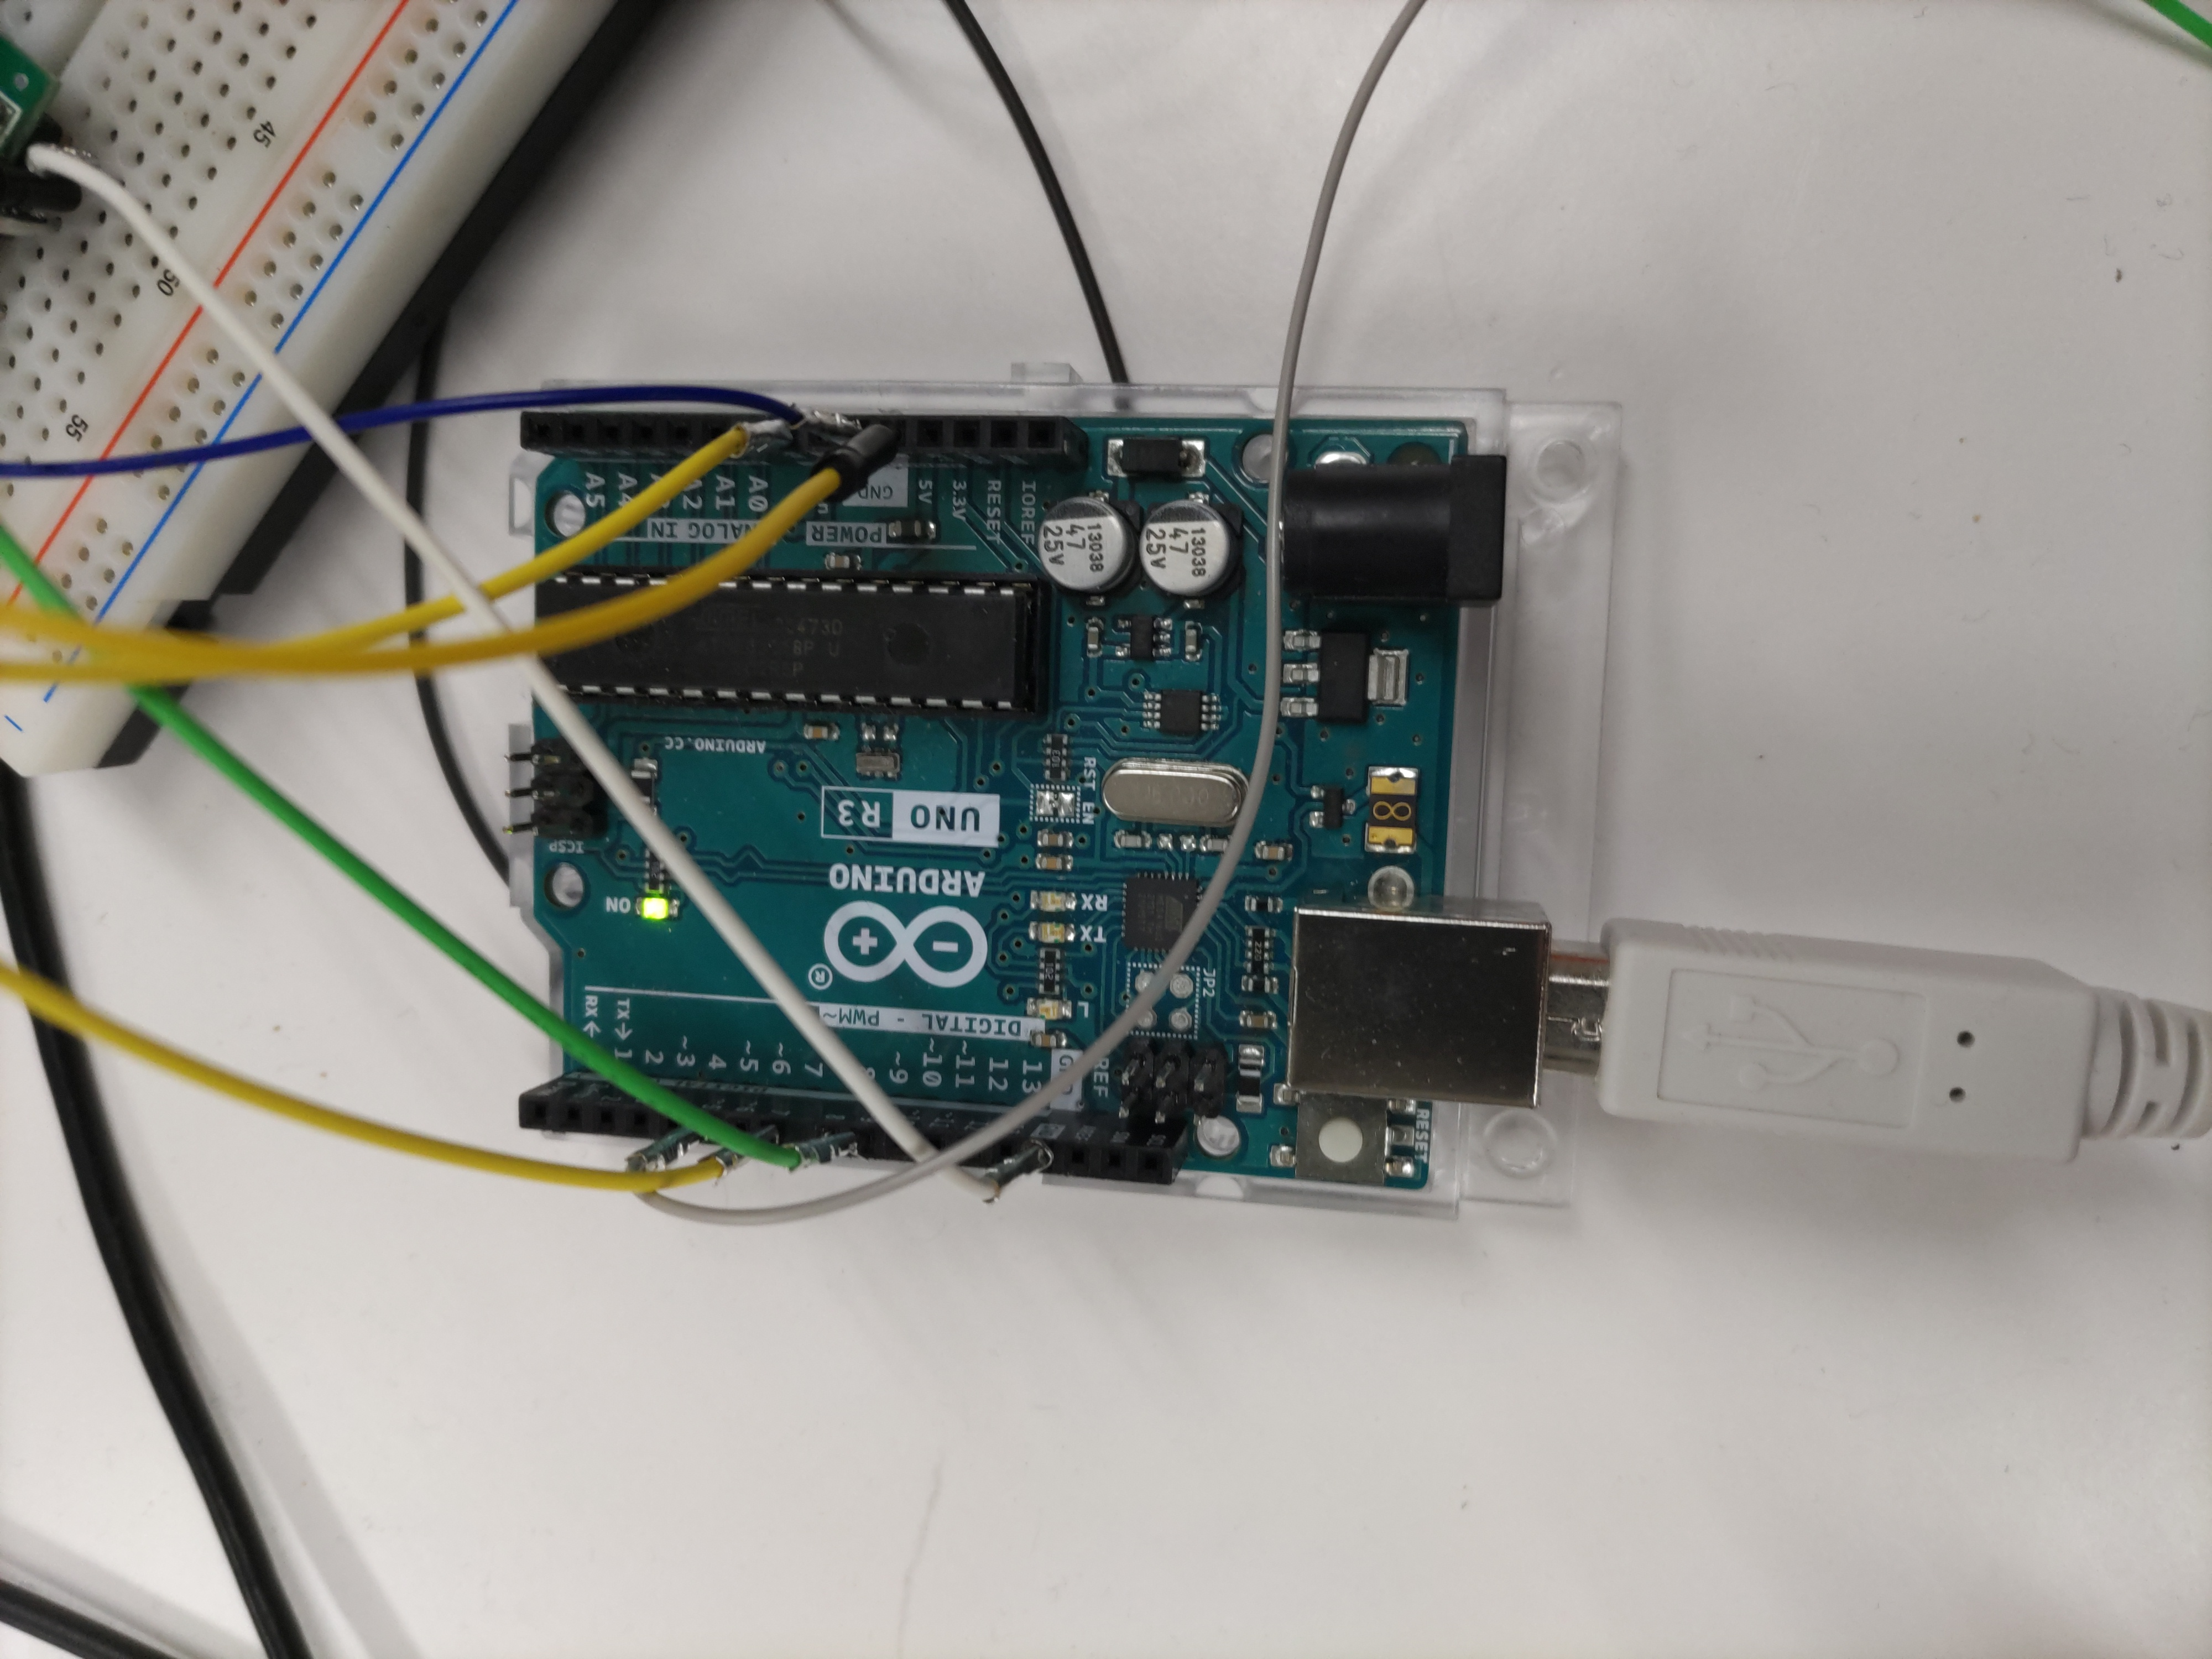
\includegraphics[clip,width=8cm]{./fig/Arduino.jpg}
\caption{Arduino UNO R3}\label{arduino}
\end{figure}

本研究で使用したArduino UNO R3を\figref{arduino}に示す.
以下,Arduino UNO R3をArduinoと記述する.

Arduino はArduino S.L.Iによって開発,販売されているマイコンである.

本研究では,押しボタンからの信号をUnity側に送信


\section{Unity}

\begin{figure}[h]
\centering
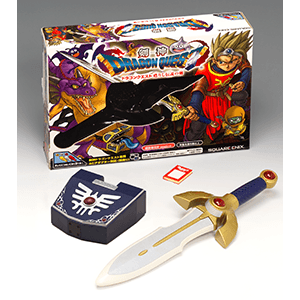
\includegraphics[clip,width=8cm]{./fig/DQN.png}
\caption{Unity上の画面}\label{unity}
\end{figure}

unityはUnity Technologies社が開発・販売しているゲームエンジンである.ゲーム開発や仮想現実,拡張現実などのアプリケーションを開発するためのゲームエンジンである.プログラミングの初心者からプロの開発者まで利用しやすいため,学習や教育の分野でも利用されている.

unityの開発画面を\figref{unity}に示す.



\section{関連研究}

\subsection{スマートフォンにおける多様な振動フィードバックが被験者の印象に与える影響}
スマートフォンにおける多様な振動フィードバックが被験者の印象に与える影響{参考入れる}の研究を白神らが行った.この研究では振動パターンがユーザーに与える印象に焦点を当て,約250通りの振動パターンからユーザーがどのような印象を持ったのかを調査したものである。

% \figref{vive}
は振動パターンの一例です。これはジョジョに振動強度が上昇するもので,この振動刺激はユーザーに力強いという印象を与えます。



しかし,この研究は,スマホという掌の上での振動でしかなく,さらに大きな物体での振動についての調査は行っていない.
また,実際に存在しているものに関する振動についての調査なので,魔法という非現実的なものに対する振動については明かされていない.





%%%%%%%%%%%%%%%%%%%%%%%%%%%%%%%%%%%%%%%%%%%%%%%%%%%%%%%%%%%%%%%%%%%%%%%
\begin{comment}
  \begin{textblock}{6.5}(1, 18)
    \noindent
    【16,18】図番号は章ごとの通し番号で抜けがない
  \end{textblock}
  
  \begin{textblock}{7}(13, 22)
    ←本文で説明がない図は載せない
  \end{textblock}
\end{comment}
%%%%%%%%%%%%%%%%%%%%%%%%%%%%%%%%%%%%%%%%%%%%%%%%%%%%%%%%%%%%%%%%%%%%%%%